%----------------------------------------------------------------------------
\chapter{Több kamerából álló kamera-rendszerek \label{chapter2}}
%----------------------------------------------------------------------------

A kitűzött feladat szempontjából két fontos részproblémát kell több kamerából álló rendszerek esetén megoldanom. Az első a kamerák szinkronizációjának problémája, ami akkor merül fel, ha a kamerák nem egy közös feldolgozó egységhez kapcsolódnak, hanem például a kamerák képeit egy videófolyamként kapjuk. A második pedig, hogy a kamerák képei alapján a háromdimenziós teret, vagy annak egy részét a lehető legjobban rekonstruáljam. Ez a fejezet ezen két problémát járja körbe, valamint végül bemutat egy megoldást a mozgó objektumok detektálására.


%----------------------------------------------------------------------------
\section{Kamerák szinkronizációja}
%----------------------------------------------------------------------------


Amennyiben a videófolyamba időpecséteket kódolunk, a kamerák szinkronizációja könnyen megoldható. A képsorokat a kódolt információ alapján egymáshoz tudjuk időzíteni, feltéve, hogy a kamerák óráit már előtte szinkronizáltuk.

Amennyiben ilyen adat nem áll rendelkezésre a videófolyamban, egyéb módszert kell keresnünk. Megoldás lehet, ha a kamerák képsorain egy közös trigger-eseményt keresünk. Egy korábbi munkám során \cite{onlab-1} egy lézerpontot kerestem mindegyik képen, és a felvillanás időpontját tekintettem referenciának. Ehhez nagyon hasonló a filmiparban használt \textit{clapperboard}, aminek összeütését használják szinkronizációra, de akár egy egyszerű taps is megfelelhet, amennyiben a kamerák hangot is rögzítenek.


%----------------------------------------------------------------------------
\section{Epipoláris geometria \label{sec:epipolar}}
%----------------------------------------------------------------------------

Az epipoláris geometria adja meg a kapcsolatot két kamera képe között \cite[9. fejezet]{HZ}. Tekintsük \aref{fig:epipolar}. ábrát. $C_1$ és $C_2$ pontok a kamerák középpontjai, és legyen $P$ egy pont a térben, mely az első kamera $I_1$ képén $p_1$-be, a második kamera $I_2$ képén $p_2$-be képződik le. $p_1$, $p_2$ és $P$ egy síkot határoz meg, jelöljük ezt $\pi$-vel. Ezen a síkon vannak rajta a kamerák középpontjaiból a képpontokon áthaladó félegyenesek is melyek $P$-ben metszik egymást. $\pi$-t a $P$-hez tartozó \textit{epipoláris sík}nak, a két kameraközéppontot összekötő egyenest \textit{bázis egyenes}nek, ennek metszéspontjait a képsíkokkal ($e_1$ és $e_2$) \textit{epipólus}oknak nevezzük. Gondoljuk meg, hogy ha $p_1$-t ismerjük és $p_2$-t szeretnénk meghatározni, akkor azt az epipoláris sík és az $I_2$ képsík metszésvonalán kell keresni, ezt a $p_1$-hez tartozó \textit{epipoláris egyenes}. Ezt a tulajdonságot tudjuk kihasználni ahhoz, hogy egy képpont párját a másik képen nem az egész síkon, hanem csak egy egyenesen kell keresnünk.


\begin{figure}[tbh]
\centering
\tdplotsetmaincoords{30}{130}
\begin{tikzpicture}[line join = round, line cap = round, >=triangle 45, tdplot_main_coords]
  
  \coordinate (O) at (0, 0, 0);
  
  % kocka
  
  \coordinate (C2) at (-3.5, -1, 1);
  \node [cross] at (C2) {};
  \node [above] at (C2) {\small $P$};
  
  % képsík
  
  \coordinate (I1) at (0, 0, 0);
  \coordinate (I2) at (0, 4, 0);
  \coordinate (I3) at (0, 4, 3);
  \coordinate (I4) at (0, 0, 3);

  \coordinate (_I1) at (-0.7, 5, 0);
  \coordinate (_I2) at (-0.7, 5, 3);
  \coordinate (_I3) at (-4.7, 5, 3);
  \coordinate (_I4) at (-4.7, 5, 0);


  \draw (I1) -- (I2);
  \draw (I2) -- (I3);
  \draw (I3) -- (I4);
  \draw (I4) -- (I1);
  
  \draw (_I1) -- (_I2);
  \draw (_I2) -- (_I3);
  \draw (_I3) -- (_I4);
  \draw (_I4) -- (_I1);

  \coordinate (UV) at (0, 1.1, 1.35);
  \node [cross] at (UV) {};
  \node [left] at (UV) {\small $p_1$};

  \coordinate (UV2) at (-2.86, 5, 1.4);
  \node [cross] at (UV2) {};
  \node [right] at (UV2) {\small $p_2$};

  % optikai tengely
  \coordinate (E1) at (0, 3.6071, 1.5);
  \coordinate (C1) at (1.5, 2, 1.5);
  \coordinate (A1) at (-1, 2, 1.5);

  \coordinate (E2) at (-1.3, 5, 1.5);
  \coordinate (C2_) at (-2.7, 6.5, 1.5);
  \coordinate (A2) at (-2.7, 4, 1.5);

  \node [below] at (C1) {\small $C_1$};
  \node [below] at (C2_) {\small $C_2$};
  \node [cross] at (E1) {};
  \node [cross] at (E2) {};
  \node [below] at (E1) {\small $e_1$};
  \node [below] at (E2) {\small $e_2$};
  
  \draw [dashed,shorten >=-20pt,shorten <=-20pt] (UV) -- (E1);
  \draw [dashed,shorten >=-20pt,shorten <=-20pt] (UV2) -- (E2);

  % leképezés
  
  \draw [dotted] (C1) -- (C2);
  \draw [dotted] (C2_) -- (C2);
  \draw [dotted] (C1) -- (C2_);
  
  \node at (-2, 2.5, 1) {$\pi$};
  
\end{tikzpicture}
\caption{Epipoláris geometria szemléltetése \label{fig:epipolar}}
\end{figure}

Az $\mathbf{F}$ fundamentális mátrix az epipoláris geometria algebrai megfeleltetése, mely az előbb említett képpontból epipoláris egyenesre történő leképezést adja meg:

\[\mathbf{l}' = \mathbf{F}\mathbf{x}\]

ahol $\mathbf{x}$ egy $X$ pont képe az egyik képsíkon, $\mathbf{l}'$ pedig a hozzá tartozó epipoláris egyenes a másik képsíkon. Legyen $\mathbf{x}'$ az $X$ képe a másik képsíkon, mivel rajta van $\mathbf{l}'$-n ezért $\mathbf{x}'^T \mathbf{l}' = 0$, tehát:

\[\mathbf{x}'^T\mathbf{F}\mathbf{x} = 0\]

Ezen mátrixegyenletből kiindulva, egymásnak megfelelő képpontpárokból kiszámolhatjuk $\mathbf{F}$-et, 8 pontpárból egy skála erejéig, 8-nál több esetén pedig legkisebb négyzetek módszerével (7 esetén pedig létezik nem-lineáris megoldás) \cite[10.1 alfejezet]{HZ}.

%----------------------------------------------------------------------------
\section{A háromdimenziós tér rekonstrukciója \label{sec:methods}}
%----------------------------------------------------------------------------


A dolgozat során két, alapvetően eltérő módszerre térek ki. Az első a sztereó-látás elvén alapszik, azaz a kamerákat párosával használva, azokat sztereó-kalibrálva alkotunk mélységképet, mely segítségével a képpontokat mélységinformációval ruházzuk fel. A második eljárás az optikai folyamok segítségével a kamerák képein meghatározza az egymásnak megfelelő pontokat, és ezekből a párosításokból háromszögelés után meghatározza a pontok világbeli koordinátáját.

\subsection{Sztereó-látás, sztereó-kalibráció}

Sztereó-kalibráció \cite{camera-calib-3d} során egy már ismert háromdimenziós objektumot használunk, és az alapján, hogy az objektum ismert pontjait a két kamera képén hol látjuk, kiszámolhatjuk a kamerák belső és külső paramétereit (lásd előző fejezet), valamint a kamerák egymáshoz való viszonyát (eltolás, forgatás). 

Amennyiben a két kamera képsíkja egybeesik, akkor a bázisegyenesek a képsíkokkal a végtelenben metszik egymást, ebből adódóan az epipoláris egyenesek párhuzamosak. Ha a két kamera közötti transzformáció csak tisztán egy $x$ tengellyel párhuzamos eltolás (standard sztereókamerák), akkor az epipoláris egyenesek az $x$ tengellyel is párhuzamosak, tehát a pontpárok keresése pusztán a képkockák egy adott sorára korlátozódik.

Mivel a gyakorlatban nehéz pontosan úgy elhelyezni a kamerákat, hogy képsíkjuk egybeessen és csak víszintes irányú eltolás legyen köztük, ezért a kamerák képeit célszerű \textit{rektifikál}ni, hogy a pontok párjait továbbra is csak egy képsoron legyen szükséges keresni. Ekkor a kamerák képeit úgy transzformáljuk, hogy a képsíkok egy képzeletbeli közös síkba essenek, lásd \aref{fig:rectification}. ábrát.

\begin{figure}[tbh]
\centering
\begin{subfigure}[b]{.49\textwidth}
\centering
\tdplotsetmaincoords{30}{130}
\begin{tikzpicture}[line join = round, line cap = round, >=triangle 45, tdplot_main_coords]
  
  % képsík
  
  \coordinate (I1) at (0, 0, 0);
  \coordinate (I2) at (0, 3, 0);
  \coordinate (I3) at (0, 3, 3);
  \coordinate (I4) at (0, 0, 3);

  \coordinate (_I1) at (-0.7, 4, 0);
  \coordinate (_I2) at (-0.7, 4, 3);
  \coordinate (_I3) at (-3.7, 4, 3);
  \coordinate (_I4) at (-3.7, 4, 0);


  \draw (I1) -- (I2);
  \draw (I2) -- (I3);
  \draw (I3) -- (I4);
  \draw (I4) -- (I1);
  
  \draw (_I1) -- (_I2);
  \draw (_I2) -- (_I3);
  \draw (_I3) -- (_I4);
  \draw (_I4) -- (_I1);

  \coordinate (C1) at (1.5, 1.5, 1.5);
  \coordinate (C2_) at (-2.2, 5.5, 1.5);

  \node [below] at (C1) {\small $C_1$};
  \node [below] at (C2_) {\small $C_2$};

  % leképezés

  \draw [dashed,shorten >=-10pt] (C1) -- (I1);
  \draw [dashed,shorten >=-10pt] (C1) -- (I2);
  \draw [dashed,shorten >=-10pt] (C1) -- (I3);
  \draw [dashed,shorten >=-10pt] (C1) -- (I4);
  \draw [dashed,shorten >=-10pt] (C2_) -- (_I1);
  \draw [dashed,shorten >=-10pt] (C2_) -- (_I2);
  \draw [dashed,shorten >=-10pt] (C2_) -- (_I3);
  \draw [dashed,shorten >=-10pt] (C2_) -- (_I4);
  
\end{tikzpicture}
\caption{Rektifikáció előtt a képsíkok}
\end{subfigure}\begin{subfigure}[b]{.49\textwidth}
\centering
\tdplotsetmaincoords{20}{90}
\begin{tikzpicture}[line join = round, line cap = round, >=triangle 45, tdplot_main_coords]
  
  % képsík
  
  \coordinate (I1) at (0, 0, 0);
  \coordinate (I2) at (0, 2, 0);
  \coordinate (I3) at (0, 2, 3);
  \coordinate (I4) at (0, 0, 3);

  \coordinate (_I1) at (0, 3, 0);
  \coordinate (_I2) at (0, 5, 0);
  \coordinate (_I3) at (0, 5, 3);
  \coordinate (_I4) at (0, 3, 3);
  
  \coordinate (S1) at (0, -0.5, -1);
  \coordinate (S2) at (0, 5.5, -1);
  \coordinate (S3) at (0, 5.5, 4);
  \coordinate (S4) at (0, -0.5, 4);

  \draw (I1) -- (I2);
  \draw (I2) -- (I3);
  \draw (I3) -- (I4);
  \draw (I4) -- (I1);
  
  \draw (_I1) -- (_I2);
  \draw (_I2) -- (_I3);
  \draw (_I3) -- (_I4);
  \draw (_I4) -- (_I1);

  \draw [dotted] (S1) -- (S2);
  \draw [dotted] (S2) -- (S3);
  \draw [dotted] (S3) -- (S4);
  \draw [dotted] (S4) -- (S1);
  
  \coordinate (C1) at (1.5, 1, 1.5);
  \coordinate (C2_) at (1.5, 4, 1.5);

  % leképezés

  \draw [dashed,shorten >=-10pt] (C1) -- (I1);
  \draw [dashed,shorten >=-10pt] (C1) -- (I2);
  \draw [dashed,shorten >=-10pt] (C1) -- (I3);
  \draw [dashed,shorten >=-10pt] (C1) -- (I4);
  \draw [dashed,shorten >=-10pt] (C2_) -- (_I1);
  \draw [dashed,shorten >=-10pt] (C2_) -- (_I2);
  \draw [dashed,shorten >=-10pt] (C2_) -- (_I3);
  \draw [dashed,shorten >=-10pt] (C2_) -- (_I4);
  
\end{tikzpicture}
\caption{Egy síkba transzformálva}
\end{subfigure}
\caption{Rektifikáció szemléltetése \label{fig:rectification}}
\end{figure}

\Aref{fig:stereo-calibration-before}. és \aref{fig:stereo-calibration-after}. ábrán látható, ahogy egy sakktábla-mintát (melynek valódi koordinátái ismertek), több szögből lefotózva a rektifikáció \cite{camera-calib-3d} előtt és után, hogy alakul a két kamera képe. A piros segéd egyenesek segítségével az is jó látható, hogy a rektifikáció után az egymásnak megfelelő rácspontok valóban egy vízszintes egyenesre esnek.

\begin{figure}[tbh]
  \centering
  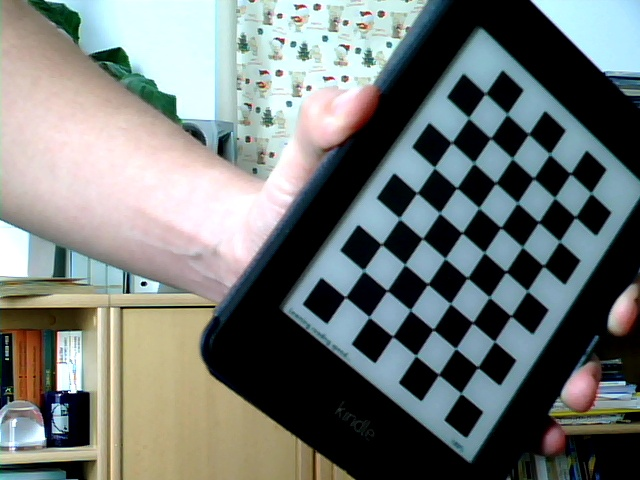
\includegraphics[width=160pt]{figures/left07.jpg}\hspace{10pt}
  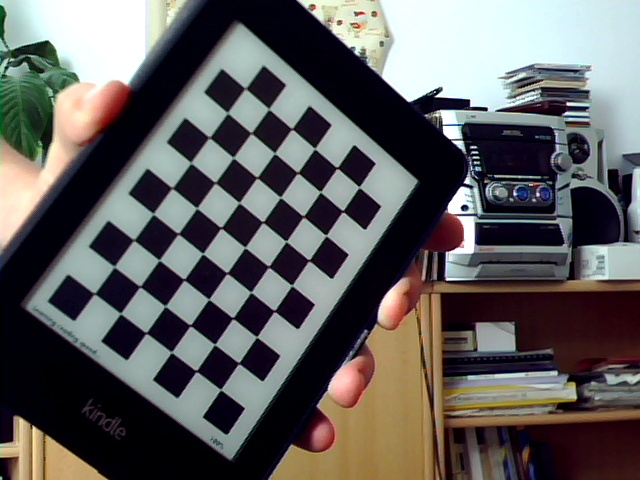
\includegraphics[width=160pt]{figures/right07.jpg}
  \caption{A kalibrációhoz felhasznált egyik képpár   \label{fig:stereo-calibration-before}}
\end{figure}

\begin{figure}[tbh]
  \centering
\begin{tikzpicture}[x=330,y=330]
	\node[anchor=south west,inner sep=0] at (0.515151,0) {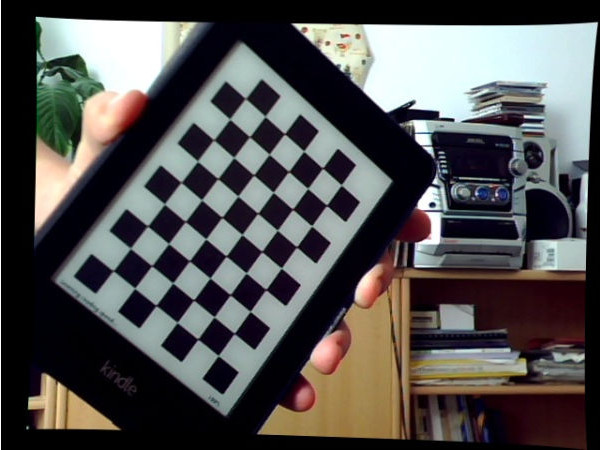
\includegraphics[width=160pt] {figures/calibrated_right.jpg}};
    \node[anchor=south west,inner sep=0] at (0,0) {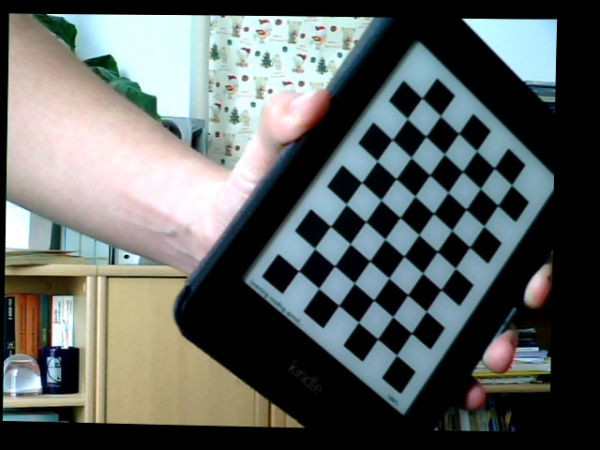
\includegraphics[width=160pt]    {figures/calibrated_left.jpg}};
    \draw[red,thick] (0,0.301) -- (1,0.301);
    \draw[red,thick] (0,0.200) -- (1,0.200);
    \draw[red,thick] (0,0.140) -- (1,0.140);
    \draw[red,thick] (0,0.045) -- (1,0.045);
\end{tikzpicture}
  \caption{Rektifikáció után a két kamera képe, pirossal jelölve néhány epipoláris egyenes \label{fig:stereo-calibration-after}}
\end{figure}

A rektifikált képpárokra pedig már léteznek algoritmusok \cite{SGBM, stereo-var}, melyek megtalálják a képeken az egymásnak megfelelő pontokat és az elmozdulásuk alapján megadják a pontok mélységértékeit. \Aref{fig:depth-showcase}. ábra segítségével könnyű látni, hogy a nagy elmozdulást mutató pontok közelebb, a kisebbek távolabb találhatóak a kamerától.

\begin{figure}[tbh]
  \centering
\begin{tikzpicture}

\tikzset{
    position label/.style={
       below = 3pt,
       text height = 1.5ex,
       text depth = 1ex
    },
   brace/.style={
     decoration={brace,amplitude=5pt},
     decorate
   }
}

  \coordinate (L1) at (0, 0);
  \coordinate (L2) at (2, 0);
  \draw (L1) -- (L2);
  
  \coordinate (C1) at (1, -1.5);
  \node [below] at (C1) {$C_1$};

  \draw [dashed, shorten >= -100pt] (C1) -- (L1);
  \draw [dashed, shorten >= -100pt] (C1) -- (L2);

  
  \coordinate (R1) at (3, 0);
  \coordinate (R2) at (5, 0);
  \draw (R1) -- (R2);
  
  \coordinate (C2) at (4, -1.5);
  \node [below] at (C2) {$C_2$};

  \draw [dashed, shorten >= -100pt] (C2) -- (R1);
  \draw [dashed, shorten >= -100pt] (C2) -- (R2);

  \coordinate (P1) at (2.5, 1.5);
  \node [cross] at (P1) {};
  \node [right] at (P1) {$P_1$};
  
  \coordinate (P2) at (2.5, 4);
  \node [cross] at (P2) {};
  \node [right] at (P2) {$P_2$};

  \draw [shorten >= -20pt] (C1) -- (P1);
  \draw [shorten >= -10pt] (C1) -- (P2);
  \draw [shorten >= -20pt] (C2) -- (P1);
  \draw [shorten >= -10pt] (C2) -- (P2);
  
  \coordinate (P2B) at (1.4090, 0);
  \node [cross] at (P2B) {};
  \node [above left] at (P2B) {$p_2'$};
  
  \coordinate (P1B) at (1.75, 0);
  \node [cross] at (P1B) {};
  \node [above right] at (P1B) {$p_1'$};
  
  \coordinate (P2J) at (3.591, 0);
  \node [cross] at (P2J) {};
  \node [above right] at (P2J) {$p_2''$};
  
  \coordinate (P1J) at (3.25, 0);
  \node [cross] at (P1J) {};
  \node [above left] at (P1J) {$p_1''$};
  
  % távolságok másolata
  
  \draw (5.5, 4) -- (7.5, 4);
  \node [cross] (T1) at (6.9090, 4) {};
  \node [cross] (T2) at (6.091, 4) {};
  \draw (5.5, 1.5) -- (7.5, 1.5);
  \node [cross] (B1) at (7.25, 1.5) {};
  \node [cross] (B2) at (5.75, 1.5) {};
  
   \draw [brace] (T1.south) -- (T2.south) node [position label, pos=0.5] {$d_2$};
   \draw [brace] (B1.south) -- (B2.south) node [position label, pos=0.5] {$d_1$};
  
\end{tikzpicture}
  \caption{Elmozdulás és mélység kapcsolata; a kameráktól távolabbi $P_2$ pont képeinek $d_2$ távolsága kisebb, mint a közelebbi $P_1$ pont képeinek $d_1$ távolsága \label{fig:depth-showcase}}
\end{figure}

Fontos megemlíteni, hogy gyakorlatban a kameráknak már eleve nagyon közel kell lenniük az ideális elhelyezkedéshez, azaz egymás mellett (vagy egymás felett, attól függően, hogy horizontális, vagy vertikális sztereó-kamerákat használunk) legyenek, úgy hogy képsíkjuk közel egybeessenek. Így érhető el az, hogy a rektifikáció sikeres legyen, valamint, hogy utána a kép legnagyobb része ,,használható'' legyen, lásd \aref{fig:stereo-calibration-after}. ábrán a képszéleken lévő fekete részeket.

\subsection{Optikai folyam \label{methods:optic}}

Az előzőekben megismert eljárás azt feltételezi, hogy a kamerák párosával sztereó-kalib\-ráltak, és ezt kihasználva határozzuk meg a mélységképet a kalibráció során alkalmazott segéd-objek\-tum alapján.

A most ismertetésre kerülő eljárás, az \textit{optikai folyam}okat \cite{optic-flow} hívja segítségül. Vegyünk egymás utáni képeket egy mozgó objektumról. Az objektum mindegyik pontja egy háromdimenziós $\mathbf{P}(t)$ útvonalon mozog, mely a kamerák képén egy $\mathbf{p}(t) = \big(x(t), y(t)\big)$ kétdimenziós útvonalnak feleltethető meg. Minden pontra nézve az elmozdulás $d\mathbf{p}(t) / dt$ irányát egy vektormezőt kapunk, ezt hívjuk optikai folyamnak.

Jelöljük $I(x, y, t)$-vel a kép $(x, y)$ pontjának intenzitását a $t$ időpillanatban. Feltehető, hogy két egymás utáni képkockán ugyanazon pont képpontjainak intenzitása konstans (\textit{világosság állandóság}, az angol \textit{brightness constancy} kifejezésből), vagyis:
\[I(x,\; y,\; t) = I(x+dx,\; y+dy,\; t+dt)\]
ahol az $(x,y)$ képpont $dt$ idő alatt $(dx,dy)$-nal mozdult el. A jobb oldal jól közelíthető az első-rendű Taylor-sor kifejtésével:

\[I(x+dx,\; y+dy,\; t+dt) \approx I(x,\; y,\; t) + \frac{\partial I}{\partial x} dx + \frac{\partial I}{\partial y} dy + \frac{\partial I}{\partial t} dt\]

Felhasználva a világosság állandóság kényszert:

\[\frac{\partial I}{\partial x} dx + \frac{\partial I}{\partial y} dy + \frac{\partial I}{\partial t} dt = 0\]

Mindkét oldalt $dt$-vel osztva:

\[\frac{\partial I}{\partial x} \frac{dx}{dt} + \frac{\partial I}{\partial y} \frac{dy}{dt} + \frac{\partial I}{\partial t} \frac{dt}{dt} = 0\]

Végül bevezetve a $\nabla \mathbf{I} = \left(\frac{\partial I}{\partial x}, \frac{\partial I}{\partial y}\right)$ és $\mathbf{V} = \left(\frac{dx}{dt}, \frac{dy}{dt}\right)$ jelöléseket, az alábbi egyszerű alakot ölti:

\[\nabla \mathbf{I} \cdot \mathbf{V} = -\frac{\partial I}{\partial t}\]

Ezt nevezzük az optikai folyam feltételi egyenletének \cite{phd}. Mivel $\mathbf{V}\left(\frac{dx}{dt}, \frac{dy}{dt}\right)$ nem ismert, ezért egy egyenletben két ismeretlenünk van, így az optikai folyam általános esetben nem oldható meg.

\subsubsection{Lucas-Kanade módszer \cite{LK}}

Ez a módszer ritka vektor-mezőt generál a jellegzetes pontok elmozdulására. Lényege, hogy a vizsgált pontok és azok környezetében az elmozdulás azonos \cite{lk-wiki}, vagyis:

\[\nabla \mathbf{I}_{\mathbf{q_1}} \cdot \mathbf{V} = -\frac{\partial I}{\partial t}(\mathbf{q_1}, t)\]
\[\nabla \mathbf{I}_{\mathbf{q_2}} \cdot \mathbf{V} = -\frac{\partial I}{\partial t}(\mathbf{q_2}, t)\]
\[\vdots\]
\[\nabla \mathbf{I}_{\mathbf{q_n}} \cdot \mathbf{V} = -\frac{\partial I}{\partial t}(\mathbf{q_n}, t)\]

ahol $\mathbf{q_1},\mathbf{q_2},\ldots,\mathbf{q_n}$ a vizsgált pont környezetében lévő pontok és $\nabla \mathbf{I}_{\mathbf{q_i}} = \left(\frac{\partial I}{\partial x}(\mathbf{q_i}), \frac{\partial I}{\partial y}(\mathbf{q_i})\right)$. Ez így viszont már egy túlhatározott egyenletrendszer, melyhez közelítő megoldás a legkisebb-négyzetek módszerével kereshető \cite{LK, lk-wiki}. A gyakorlatban a követendő pontokra a Shi-Thomasi \cite{shi-thomasi} módszer által adott sarokpontokat szokták használni (lásd \aref{fig:lk}. ábra).

\begin{figure}[tbh]
\centering
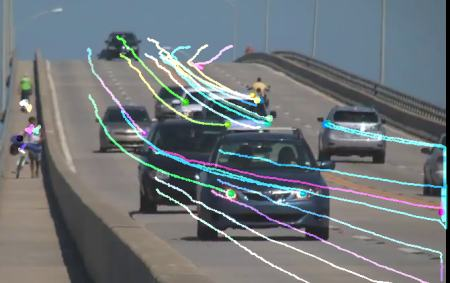
\includegraphics[width=300pt]{figures/opticalflow_lk.jpg}
\caption{Minta a sarokpontok követésére \cite{opencv-lk} \label{fig:lk}}
\end{figure}

\subsubsection{Gunner Farnebäck módszer \cite{farneback}}

A módszer lényege, hogy a kép pixeleinek intenzitását egy polinommal közelíti:

\[f(\mathbf{x}) \sim \mathbf{x}^T \mathbf{A} \mathbf{x} + \mathbf{b}^T \mathbf{x} + c\]

ahol $\mathbf{A}$ egy szimmetrikus mátrix, $\mathbf{b}$ vektor és $c$ skalár.

Ezeket az együtthatókat a legkisebb-négyzetek módszerével közelítően meghatározhatjuk. Tegyük fel, hogy mindkét kép összes pixelének intenzitása egyetlen polinommal felírható, és a két képkockán az egész polinom ideálisan $\mathbf{d}$-vel mozdul el, vagyis:

\[f_1(\mathbf{x} - \mathbf{d}) = f_2(\mathbf{x})\]

A fenti képlet jelenti a világosság állandóság kényszer teljesülését. Bal oldalt kifejtve, jobb oldalt pedig átírva a polinom-alakba \cite{farneback}:

\[\mathbf{x}^T \mathbf{A}_1 \mathbf{x} + (\mathbf{b_1} - 2 \mathbf{A}_1\mathbf{d})^T \mathbf{x} + \mathbf{d}^T \mathbf{A}_1 \mathbf{d} -\mathbf{b}_1^T + c_1 = \mathbf{x}^T \mathbf{A}_2 \mathbf{x} + \mathbf{b_2}^T \mathbf{x} + c_2\]

Az együtthatókat egyenlővé téve, kapjuk a következő egyenleteket:

\[\begin{array}{rcl}\mathbf{A}_2 &=& \mathbf{A}_1\\\mathbf{b_2} &=& \mathbf{b_1} - 2 \mathbf{A}_1\mathbf{d}\\ c_2 &=& \mathbf{d}^T \mathbf{A}_1 \mathbf{d} -\mathbf{b}_1^T + c_1 \end{array}\]

Jól látható, hogy $\mathbf{d}$ meghatározható ha $\mathbf{A}_1$ determinánsa nem nulla. Általános esetben természetesen nem élhetünk az előbbi feltételekkel, miszerint mindkét kép leírható egyetlen polinommal és ideálisan minden pont $\mathbf{d}$-vel mozdult el. Ezért lokális polinomokkal dolgozunk, melyek a pontok egy környezetében érvényesek, vagyis $\mathbf{A}_1(\mathbf{x}), \mathbf{b_1}(\mathbf{x}),$ $c_1(\mathbf{x})$ és $\mathbf{A}_2(\mathbf{x}), \mathbf{b_2}(\mathbf{x}), c_2(\mathbf{x})$ együtthatókkal kell számolunk. Ekkor az alábbi közelítéseket téve:
\[\mathbf{A}(\mathbf{x}) = \frac{\mathbf{A}_2(\mathbf{x}) + \mathbf{A}_2(\mathbf{x})}{2}\]
\[\Delta \mathbf{b}(\mathbf{x}) = -\frac{1}{2}\left(\mathbf{b}_2(\mathbf{x})-\mathbf{b}_1(\mathbf{x})\right)\]
Kapjuk az előbbi egyenletekkel összevetve a következőt:
\[\mathbf{A}(\mathbf{x})\mathbf{d}(\mathbf{x}) = \Delta \mathbf{b}(\mathbf{x})\]

Ekkor $\mathbf{d}(\mathbf{x})$ szerepében megkaptuk a vektor-mezőt. Ez az egyenlet pontonként felírva megoldható, de a gyakorlatban zajos eredményt szolgáltat. Ezt elkerülendő azzal a feltevéssel élünk, hogy a pontok egy környezetében az elmozdulás vektorok csak kicsit változnak, és így a fenti megoldása egy költség-minimalizálási problémává változik \cite{farneback}.

Ez utóbbi algoritmust \cite{opencv-lk} választottam a feladat megoldása során, mert sűrű optikai folyamokat szolgáltat, és nem kell sarokpontokat keresni a kiinduló képen. \Aref{fig:dense-of}. ábrán látható egy példa, ami egy kanyon felett elrepülő helikopter videójának két egymás utáni képkockájából meghatározott sűrű optikai folyamot mutatja. Fontos megemlíteni, hogy mindkét eljárás önmagában csak kis mozgásokat tud követni, ezért nagy elmozdulások esetén a piramis-módszert használjuk: a képeket több lépcsőben kicsinyítjük, és ezeken is lefuttatjuk az algoritmusokat, így a kis mozgások eltűnnek, a nagyok pedig kisebbekké, ezáltal detektálhatóvá válnak.

\begin{figure}[tbh]
\centering
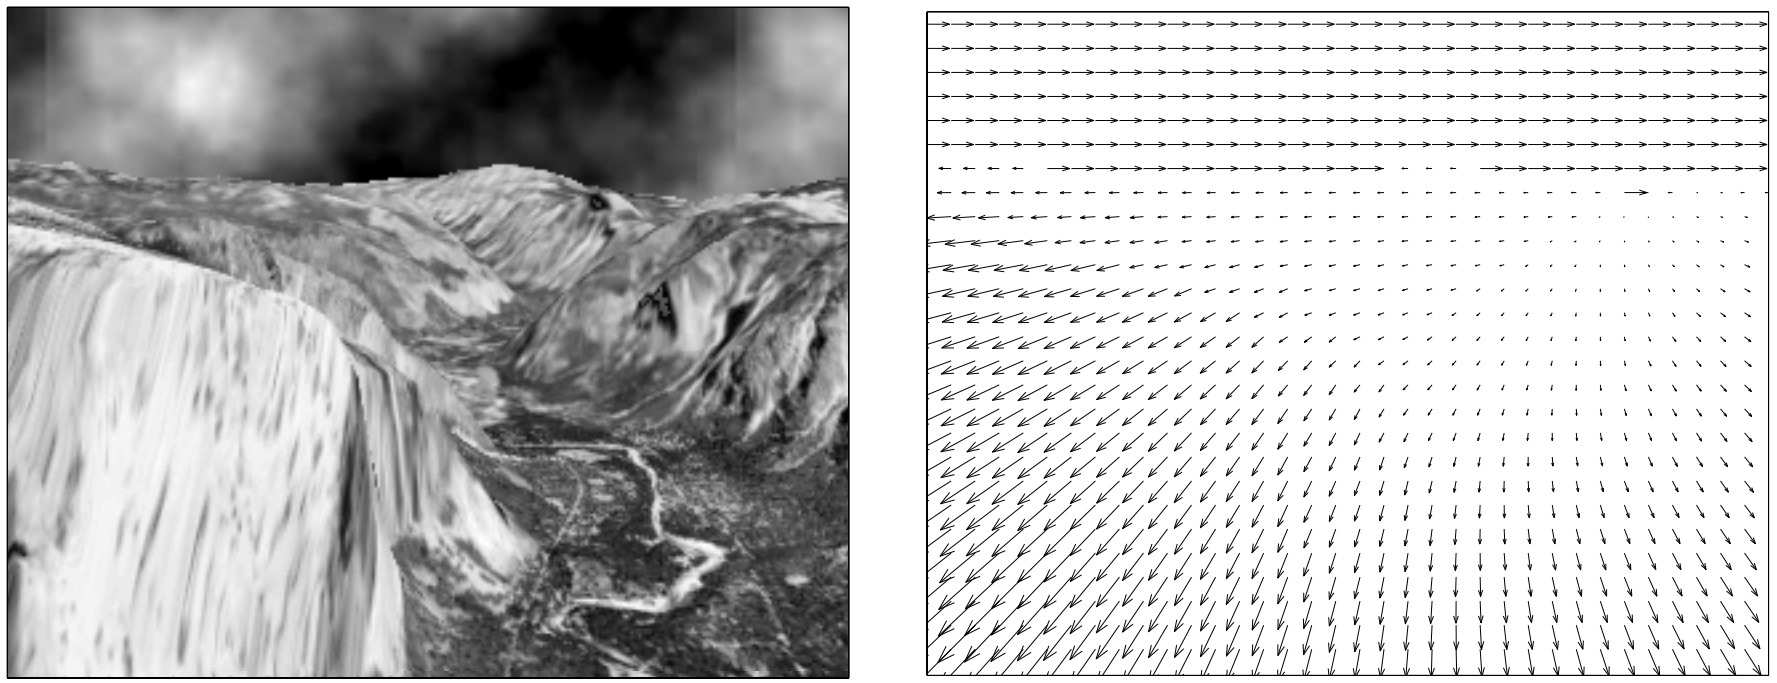
\includegraphics[width=420pt]{figures/farneback.png}
\caption{Minta sűrű optikai folyam meghatározásra \cite{farneback} \label{fig:dense-of}}
\end{figure}

Az optikai folyamokat felhasználhatjuk statikus objektumok (pl. szobrok, kastélyok) modellezésére, ezt a problémát \textit{structure-from-motion}-nek hívjuk \cite{sfm}. Tekintsünk egy adott objektum felé néző, de körülötte mozgó kamera két helyzetében ($C_1$ és $C_2$) látott képet (lásd \aref{fig:triangulation}. ábrát). Az objektumról a kamera mozgása során több képet készítve, és ezeken az egymásnak megfelelő pontokat az optikai folyamok segítségével meghatározva a már említett háromszögelés módszerével meghatározhatóak a pontok háromdimenziós koordinátái, valamint a nézőpontok közötti transzformációk is \cite[4. fejezet]{book}.

\begin{figure}[tbh]
\centering
\tdplotsetmaincoords{60}{130}
\begin{tikzpicture}[line join = round, line cap = round, >=triangle 45, tdplot_main_coords]
  
  \coordinate (O) at (0, 0, 0);
  
  % kocka
  
  \coordinate (C1) at (-4.5, -2, 1);
  \coordinate (C2) at (-4.5, -1, 1);
  \coordinate (C3) at (-4.5, -1, 2);
  \coordinate (C4) at (-4.5, -2, 2);
  \coordinate (C1B) at (-5, -2, 1);
  \coordinate (C2B) at (-5, -1, 1);
  \coordinate (C3B) at (-5, -1, 2);
  \coordinate (C4B) at (-5, -2, 2);
    \node [below right] at (C2) {\small $(X, Y, Z)$};

  \draw [dashed] (C1) -- (C2);
  \draw [dashed] (C2) -- (C3);
  \draw [dashed] (C3) -- (C4);
  \draw [dashed] (C4) -- (C1);
  \draw [dashed] (C1) -- (C1B);
  \draw [dashed] (C2) -- (C2B);
  \draw [dashed] (C3) -- (C3B);
  \draw [dashed] (C4) -- (C4B);
  \draw [dashed] (C1B) -- (C2B);
  \draw [dashed] (C2B) -- (C3B);
  \draw [dashed] (C3B) -- (C4B);
  \draw [dashed] (C4B) -- (C1B);
  
  
  % képsík
  
  \coordinate (I1) at (0, 0, 0);
  \coordinate (I2) at (0, 4, 0);
  \coordinate (I3) at (0, 4, 3);
  \coordinate (I4) at (0, 0, 3);

  \coordinate (_I1) at (-0.7, 5, 0);
  \coordinate (_I2) at (-0.7, 5, 3);
  \coordinate (_I3) at (-4.7, 5, 3);
  \coordinate (_I4) at (-4.7, 5, 0);


  \draw (I1) -- (I2);
  \draw (I2) -- (I3);
  \draw (I3) -- (I4);
  \draw (I4) -- (I1);
  
  \draw (_I1) -- (_I2);
  \draw (_I2) -- (_I3);
  \draw (_I3) -- (_I4);
  \draw (_I4) -- (_I1);

  \coordinate (UV) at (0, 0.421, 1.2368);
  \node [cross] at (UV) {};

  \coordinate (UV2) at (-3.5182, 5, 1.2727);
  \node [cross] at (UV2) {};

  % optikai tengely
  \coordinate (P1) at (0, 2, 1.5);
  \coordinate (C1) at (5, 2, 1.5);
  \coordinate (A1) at (-1, 2, 1.5);

  \coordinate (P2) at (-2.7, 5, 1.5);
  \coordinate (C2_) at (-2.7, 10, 1.5);
  \coordinate (A2) at (-2.7, 4, 1.5);

  \node [below] at (C1) {\small $C_1$};
  \node [below] at (C2_) {\small $C_2$};
  \draw (C1) -- (P1);
  \draw (C2_) -- (P2);
  \node [cross] at (P1) {};
  \node [cross] at (P2) {};
  \node [below right] at (P1) {\small $P_1$};
  \node [below left] at (P2) {\small $P_2$};
  \draw [dashed,-latex] (P1) -- (A1);
  \draw [dashed,-latex] (P2) -- (A2);
  
  % leképezés
  
  \draw [dotted] (C1) -- (C2);
  \draw [dotted] (C2_) -- (C2);
  
  \draw [shorten <= 10pt, shorten >= 10pt,dashed,->,>=stealth'] (C1) to[out=-20,in=-160] (C2_);
  
\end{tikzpicture}
\caption{Mozgó kamera két állapotban \label{fig:triangulation}}
\end{figure}

Ennél lényegesen eltérő felhasználási mód, ha az optikai folyamokat nem egy mozgó kamera két képkockáján, hanem két különböző kamera egy időponthoz tartozó két képkockáján határozzuk meg, melyek megközelítőleg ugyanazon térrészt veszik, de kissé eltérő pontból és szögből. Ekkor az optikai folyam lényegében a két kamera képén egy megfeleltetést tesz lehetővé. Feltéve, hogy előzetesen a kamerák pozícióját meghatároztuk (külső paraméterek), valamint ismerjük a projekciójukat leíró mátrixokat (belső paraméterek), akkor az egyező képontokat felhasználva háromszögeléssel kaphatjuk a mindkét kamera által látott pontok világbeli koordinátáit.

Az előbbi módszer jól használható nagy felbontású képeknél, ahol az objektum a kép nagy részét teszi ki, és így sok hasznos képpontot gyűjthetünk. A feladatom során éppen ellenkezőleg, a képek csak egy részén megjelenő és ott mozgó objektumokat kellett rekonstruálni, így az utóbbi megközelítést valósítottam meg.


%----------------------------------------------------------------------------
\subsection{Háromszögelés \label{sec:triangulation}}
%----------------------------------------------------------------------------

Legyen adott két kamera a belső és külső paramétereivel együtt, tehát ismerjük a kamerák $\mathbf{P}$ és $\mathbf{Q}$ projekciós mátrixát. Amennyiben vesszük egy $P$ pont vetületeit a kamerák képein, akkor háromszögeléssel meghatározhatjuk ezen pont valóvilágbeli koordinátáit.

Legyen a két egymásnak megfeleltetett képpont $\mathbf{u}$ és $\mathbf{u}'$. A megfeleltetés zajos jellege miatt, ezek általánosságban nem elégítik ki az epipoláris $\mathbf{u}'^T \mathbf{F} \mathbf{u} = 0$ kényszert, ahol $\mathbf{F}$ a két kamera fundamentális mátrixa. Ilyenkor ezek helyett olyan $\mathbf{\hat{u}} \leftrightarrow \mathbf{\hat{u}}'$ megfeleltetést keresünk, mely minimalizálja az alábbi

\[d(\mathbf{u}, \mathbf{\hat{u}})^2 + d(\mathbf{u}', \mathbf{\hat{u}}')^2\]

költségfüggvényt, ahol $d(., .)$ két pont euklideszi távolsága, és kielégíti az

\[\mathbf{\hat{u}}'^T \mathbf{F} \mathbf{\hat{u}} = 0\]

epipoláris kényszert \cite{hartley-triangulation}. Amikor megvan $\mathbf{\hat{u}}$ és $\mathbf{\hat{u}}'$, már meghatározhatjuk a kameraközéppontokból induló ezen pontokon átmenő sugarak metszéspontjait, hiszen biztosan létezni fog. Hartley és Sturm \cite{hartley-triangulation} megad egy optimális polinomiális megoldást, mely a fenti költségfüggvényt minimalizálja Gauss-eloszlású zaj feltételezése esetén.

Ennek ellenére a gyakorlatban inkább lineáris háromszögelést szoktak alkalmazni \cite[5.1 szekció]{hartley-triangulation}. Legyen $\mathbf{x}$ egy pont és ennek vetülete az első kamera képén $\mathbf{u}$, vagyis $\mathbf{u} = \mathbf{P}\mathbf{x}$. Legyen $\mathbf{u}$ homogén koordinátákkal $\mathbf{u} = w_u[x_u, y_u, 1]^T$, tehát:

\[w_u\left[ \begin{array}{c} x_u \\ y_u \\ 1 \end{array} \right] = \left[ \begin{array}{c} \mathbf{p}_1^T \\ \mathbf{p}_2^T \\ \mathbf{p}_3^T \end{array} \right] \mathbf{x}\]

ahol $\mathbf{p}_i^T$ jelöli a $\mathbf{P}$ mátrix $i$. sorvektorát. Így összesen 3 egyenletet kapunk:

\[w_ux_u = \mathbf{p}_1^T\mathbf{x} \quad w_uy_u = \mathbf{p}_2^T\mathbf{x} \quad w_u = \mathbf{p}_3^T\mathbf{x}\]

Harmadik egyenlőséget felhasználva az első kettőnél, kapjuk, hogy:

\[x_u\mathbf{p}_3^T\mathbf{x} = \mathbf{p}_1^T\mathbf{x}\]
\[y_u\mathbf{p}_3^T\mathbf{x} = \mathbf{p}_2^T\mathbf{x}\]

Ugyanezt levezetve $\mathbf{v} = w_v[x_v, y_v, 1]^T = \mathbf{Q}\mathbf{x}$ képpontra:

\[x_v\mathbf{q}_3^T\mathbf{x} = \mathbf{q}_1^T\mathbf{x}\]
\[y_v\mathbf{q}_3^T\mathbf{x} = \mathbf{q}_2^T\mathbf{x}\]

A fenti négy egyenletet rendezve:

\[\left( \begin{array}{c} x_u\mathbf{p}_3^T - \mathbf{p}_1^T \\ y_u\mathbf{p}_3^T - \mathbf{p}_2^T \\ x_v\mathbf{q}_3^T - \mathbf{q}_1^T \\ y_v\mathbf{q}_3^T - \mathbf{q}_2^T \end{array} \right) \mathbf{x} = 0\]

Ez meghatározza $\mathbf{x}$-et egy faktor erejéig, és ennek nem-zérus megoldását keressük. Zajos adatokat feltételezve ennek nem feltétlen találunk pontos megoldást, így közelítenünk kell. Egy lehetséges megközelítés a \textit{Linear-LS} (lineáris, legkisebb négyzetek) módszer, mely $\mathbf{x} = [x, y, z, 1]^T$ alakú megoldások között keresi az egyenletrendszer legkisebb négyzetek megoldását (pl. szinguláris érték szerinti felbontással (SVD) \cite{cs-svd}). 

Általános esetben a talált $\mathbf{x}$ nem pontos megoldása a fenti egyenleteknek, azaz egy $\varepsilon = x_u\mathbf{p}_3^T\mathbf{x} - \mathbf{p}_1^T\mathbf{x}$ hibával számolhatunk az egyenletrendszer első egyenleténél. Mi nem ezt, hanem $x_u$ és $\mathbf{x}$ vetületének első koordinátája közötti eltérését szeretnénk minimalizálni, azaz $\varepsilon' = \frac{\varepsilon}{\mathbf{p}_3^T\mathbf{x}} = x_u - \frac{\mathbf{p}_1^T\mathbf{x}}{\mathbf{p}_3^T\mathbf{x}}$. Tehát, ha az egyenletet $1 / \mathbf{p}_3^T\mathbf{x}$-szel súlyoztuk volna, akkor az úgy kapott hiba pont az általunk minimalizálandó hiba lett volna. Természetesen ezt nem tudjuk megtenni, hiszen $\mathbf{x}$ még nem ismert, csak miután megoldottuk az egyenletrendszert, de egy iteratív megközelítést tudunk alkalmazni. Minden iteráció végén újrasúlyozzuk a megfelelő sorokat $1 / \mathbf{p}_3^T\mathbf{x}_i$, valamint $1 / \mathbf{q}_3^T\mathbf{x}_i$-vel, ahol $\mathbf{x}_i$ az $i$. iteráció végén kapott megoldás. Ha a lépéseknél az aktuális megoldást az előbbi \textit{Linear-LS}-sel keressük, akkor az így kapott eljárást \textit{Iterative-LS}-nek hívjuk. Hartley és Sturm \cite[5.2 szekció]{hartley-triangulation} munkája alapján az esetek 95\%-ban a megoldás konvergens (epipólus melletti pontokra volt divergens), és amikor az új súly már csak kis mértékben változik az előzőhöz képest, megszakíthatjuk az iterációt.

%----------------------------------------------------------------------------
\section{Objektum-detektálás \label{sec:obj_detection}}
%----------------------------------------------------------------------------

Objektumok detektálására a szakirodalomban több eltérő módszert is találhatunk. Az egyik legegyszerűbb ezek közül a minta alapú illesztés (\textit{feature matching}) \cite{brunelli1997template}. Ekkor lényegében egy minta képet illesztünk egy forrás képre csúszóablakos módszerrel, és valamely metrika mentén minden pozícióban egy illeszkedési értéket számolunk. Ezt az egész képre meghatározva, majd ennek ennek a maximumát véve kapjuk az illeszkedési pontot, ahol a keresett objektumot megtaláltuk.

Egy másik nagyon elterjedt módszer a kaszkád osztályozó (\textit{cascade classifier}), ami gépi tanuláson alapszik \cite{viola2001rapid}. Ennek segítségével egy előzetes tanulási szakasz után viszonylag komplex objektumok felismerése is nagyon gyorsan lehetővé válik.

A harmadik módszer, amit kiemelnék a jellegzetes pontok megfeleltetésén (\textit{feature matching}) alapszik. A keresendő objektumon és a forrás képen különböző algoritmusok segítségével jellegzetes pontokat emelünk ki, majd ezek tulajdonságait egy leíróban tároljuk, végül ezeket egymásnak a két képen megfeleltetjük, párosítjuk és a legnagyobb egyezőség

\subsection{Mozgó objektumok kiválasztása}
%----------------------------------------------------------------------------

Mivel a feladat megoldása során mozgó objektumokat kell követnem, azokat modelleznem, így szükség van a mozgó objektumok statikus háttértől való elkülönítésére.

Egy lehetőségünk például az előző részben leírt Farnebäck-módszer használata. Egy kamera egymás utáni képkockáira alkalmazva, becslést kaphatunk arra vonatkozóan, hogy hol lehetnek a mozgó tárgyak. A kamerák statikus helyzete révén, a háttér képpontjaihoz tartozóan közel zéró elmozdulást várunk, míg a mozgó részeken ettől eltérőt.

Másik megoldás lehet például egy háttér-előtér szegmentálási algoritmus (MOG) \cite{MOG}, mely az egymás utáni képkockákból egy háttér-modellt épít. Az aktuális képkockából a kapott hátteret kivonva, megkapjuk az éppen aktuális előtérhez tartozó maszkot, lásd \aref{fig:mog-example}. ábrát. Ezen algoritmus előnye, hogy az árnyékokat nagy valószínűséggel kiszűrí, és azokat nem tekinti az objektum részének, valamint a folyamatos modellépítésnek köszönhetően, nem csak egy fix tanulási időszak alatt gyűjtött információkból határozza meg a hátteret.

\begin{figure}[tbh]
\centering
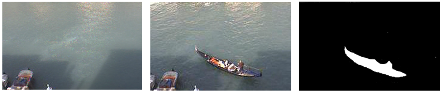
\includegraphics{figures/mog.png}
\caption{Minta a háttér-előtér elválasztási algoritmus eredményére \cite{mog-example} \label{fig:mog-example}}
\end{figure}

\subsection{Objektumok meghatározása a kamerák képein}
%----------------------------------------------------------------------------

Miután meghatároztam a mozgó objektumokhoz tartozó maszkokat, az ezek által kijelölt képrészleteket kell úgy párosítanom a kamerák képein, hogy azok egy valódi objektumhoz tartozzanak.

Erre a feladatra a kaszkád osztályozót a szükséges előzetes tanítás miatt elvetettem. A minta alapú illesztést alkalmazhattam volna úgy, hogy az egyik képen meghatározott képrészleteket egyenként használom a másik kép számára mintaként. Ahogy majd később látni fogjuk az optikai folyam alapú sűrű pont-pont megfeleltetés robosztus meghatározásához szükségünk lesz előzetes megfeleltetésre, ezért az előző fejezetben leírt objektumok detektálásához használható eljárások közül a jellegzetes pont alapú megfeleltetését választottam. Ennek segítségével az előtérhez tartozó képrészleteket párosítottam a kamerák képein, így sikeresen detektáltam a mozgó objektumokat a kamerák képein.

%----------------------------------------------------------------------------
\section{Összefoglaló}
%----------------------------------------------------------------------------

Ebben a fejezetben a több kamerából álló kamera-rendszerek során felmerülő és a dolgozat során is megoldandó problémákat, valamint ezek lehetséges megoldásait mutattam be. Kitértem a kamerák szinkronizációjára, az epipoláris geometriára, mely kapcsolatot teremt a kamerák képei között, és leírtam két lényegében eltérő rekonstrukciós eljárást, és azok mögött meghúzódó elméleti hátteret. Bemutattam a háromszögelés elméleti módszerét, végül a fejezetet az objektum-detektálás problémakörével zártam.